%%
%% This is file `mcmthesis-demo.tex',
%% generated with the docstrip utility.
%%
%% The original source files were:
%%
%% mcmthesis.dtx  (with options: `demo')
%%
%% -----------------------------------
%%
%% This is a generated file.
%%
%% Copyright (C)
%%       2010 -- 2015 by Zhaoli Wang
%%       2014 -- 2019 by Liam Huang
%%       2019 -- present by latexstudio.net
%%
%% This work may be distributed and/or modified under the
%% conditions of the LaTeX Project Public License, either version 1.3
%% of this license or (at your option) any later version.
%% The latest version of this license is in
%%   http://www.latex-project.org/lppl.txt
%% and version 1.3 or later is part of all distributions of LaTeX
%% version 2005/12/01 or later.
%%
%% This work has the LPPL maintenance status `maintained'.
%%
%% The Current Maintainer of this work is Liam Huang.
%%
%%
%% This is file `mcmthesis-demo.tex',
%% generated with the docstrip utility.
%%
%% The original source files were:
%%
%% mcmthesis.dtx  (with options: `demo')
%%
%% -----------------------------------
%%
%% This is a generated file.
%%
%% Copyright (C)
%%       2010 -- 2015 by Zhaoli Wang
%%       2014 -- 2019 by Liam Huang
%%       2019 -- present by latexstudio.net
%%
%% This work may be distributed and/or modified under the
%% conditions of the LaTeX Project Public License, either version 1.3
%% of this license or (at your option) any later version.
%% The latest version of this license is in
%%   http://www.latex-project.org/lppl.txt
%% and version 1.3 or later is part of all distributions of LaTeX
%% version 2005/12/01 or later.
%%
%% This work has the LPPL maintenance status `maintained'.
%%
%% The Current Maintainer of this work is Liam Huang.
%%
\documentclass{mcmthesis}
\mcmsetup{CTeX = false,    % 使用 CTeX 套装时，设置为 true
          tcn = {2517063}, problem = \textcolor{red}{C},
          sheet = true, titleinsheet = true, keywordsinsheet = true,
          titlepage = false, abstract = false}
        
\usepackage{newtxtext}     % \usepackage{palatino}
\usepackage[backend=bibtex]{biblatex}   % for RStudio Complie
\usepackage{booktabs}
\usepackage{colortbl}
\usepackage{underscore}
\usepackage{tocloft}
\usepackage{float}
\usepackage{enumitem}

\setlength{\cftbeforesecskip}{6pt}
\renewcommand{\contentsname}{\hspace*{\fill}\Large\bfseries Contents \hspace*{\fill}}

\title{Enjoy a Cozy and Green Bath}
% \author{\small \href{http://www.latexstudio.net/}
%   {\includegraphics[width=7cm]{mcmthesis-logo}}}
\date{\today}

\begin{document}

\begin{abstract}

A traditional bathtub cannot be reheated by itself, so users have to add hot water from time to time. Our goal is to establish a model of the temperature of bath water in space and time. Then we are expected to propose an optimal strategy for users to keep the temperature even and close to initial temperature and decrease water consumption.

To simplify modeling process, we firstly assume there is no person in the bathtub. We regard the whole bathtub as a thermodynamic system and introduce heat transfer formulas.

We establish two sub-models: adding water constantly and discontinuously. As for the former sub-model, we define the mean temperature of bath water. Introducing Newton cooling formula, we determine the heat transfer capacity. After deriving the value of parameters, we deduce formulas to derive results and simulate the change of temperature field via CFD. As for the second sub-model, we define an iteration consisting of two process: heating and standby. According to energy conservation law, we obtain the relationship of time and total heat dissipating capacity. Then we determine the mass flow and the time of adding hot water. We also use CFD to simulate the temperature field in second sub-model.

In consideration of evaporation, we correct the results of sub-models referring to some scientists' studies. We define two evaluation criteria and compare the two sub-models. Adding water constantly is found to keep the temperature of bath water even and avoid wasting too much water, so it is recommended by us.

Then we determine the influence of some factors: radiation heat transfer, the shape and volume of the tub, the shape/volume/temperature/motions of the person, the bubbles made from bubble bath additives. We focus on the influence of those factors to heat transfer and then conduct sensitivity analysis. The results indicate smaller bathtub with less surface area, lighter personal mass, less motions and more bubbles will decrease heat transfer and save water.

Based on our model analysis and conclusions, we propose the optimal strategy for the user in a bathtub and explain the reason of uneven temperature throughout the bathtub. In addition, we make improvement for applying our model in real life.

\begin{keywords}
Heat transfer; Thermodynamic system; CFD; Energy conservation
\end{keywords}

\end{abstract}

\maketitle

%% Generate the Table of Contents, if it's needed.
% \renewcommand{\contentsname}{\centering Contents}
\tableofcontents   % 若不想要目录, 注释掉该句
\thispagestyle{empty}

\newpage

\section{Introduction}

\subsection{Problem Background}

The Olympic Games is one of the most influential sporting events globally. It not only showcases the outstanding talents of athletes but also promotes cultural exchanges and cooperation among nations. Since the revival of the modern Olympics in 1896, the Games has become an important platform for countries to display their athletic prowess. The medal table has always been an integral part of the Olympics, reflecting not only the sports levels of different countries but also being closely related to their economic, social, and cultural development. The number and rank of medals are often seen as one of the symbols of a country's comprehensive national strength. The medal table of the 2024 Paris Olympics shows the competitive landscape of countries in terms of gold medals and total medals. For example, the United States ranked first in total medals, while China and the United States were tied for first in gold medals. The host country, France, also performed well, ranking fourth. In addition, some countries such as Albania, Cabo Verde, Dominica, and Saint Lucia won medals for the first time in the Olympics, which reflected the diversity and inclusiveness of the Games.

(figure) (figure)

\subsection{Restatement of the Problem}

{\bf Question 1: Development of the Medal Quantity Prediction Model} 

$\star$ Develop a model to predict the number of medals (at least including gold medals and total medals) that each country will win at the 2028 Los Angeles Olympics. In addition, assess the uncertainty and prediction accuracy of the model, and provide prediction intervals.

$\star$ Predict which countries may improve in 2028 and which may perform worse than in 2024.

$\star$ Consider countries that have not yet won medals, and predict how many countries may win medals for the first time in 2028, along with probability estimates.

$\star$ The model should also explore the relationship between the setting of Olympic events and the medal-winning situations of various countries, and discuss the impact of the host country's event selection on the medal table. Identify which sports contribute the most to the medal counts of different countries and explain the reasons.

{\bf Question 2: "Great Coach" Effect Analysis}

$\star$ Identify the impact of "great coach" on the number of medals through data analysis.

$\star$ Estimate the proportion of this effect on the number of medals.

$\star$ Select three countries and analyze which sports they require the introduction of  "great coach", and estimate the potential impact.

{\bf Question 3:Other Original Insights}

$\star$ Provide other original insights revealed by the model regarding the Olympic medal table.

$\star$ Explain how these insights can provide decision support for country Olympic Committees.

\subsection{Literature Review}

\subsection{Our Work}
XXXXX

(figure)

\section{Assumptions and Justification}

To simplify the problem and make it convenient for us to simulate real-life conditions, we make the following basic assumptions, each of which is properly justified.

$  \blacklozenge $  {\bf Assumption 1: XXXXX.}

{\bf Justification:} XXXXX

$  \blacklozenge $  {\bf Assumption 2: XXXXX.}

{\bf Justification:} XXXXX

$  \blacklozenge $  {\bf Assumption 3: XXXXX.}

{\bf Justification:} XXXXX

$  \blacklozenge $  {\bf Assumption 4: XXXXX.} 

{\bf Justification:} XXXXX

\section{Notations}

\begin{center}
\begin{tabular}{clc}
{\bf Symbols} & {\bf Description} & \quad {\bf Unit} \\[0.25cm]
$h$ & Convection heat transfer coefficient & \quad W/(m$^2 \cdot$ K) 
\\[0.2cm]
$k$ & Thermal conductivity & \quad W/(m $\cdot$ K) \\[0.2cm]
$c_p$ & Specific heat & \quad J/(kg $\cdot$ K) \\[0.2cm]
$\rho$ & Density & \quad kg/m$^2$ \\[0.2cm]
$\delta$ & Thickness & \quad m \\[0.2cm]
$t$ & Temperature & \quad $^\circ$C, K \\[0.2cm]
$\tau$ & Time & \quad s, min, h \\[0.2cm]
$q_m$ & Mass flow & \quad kg/s \\[0.2cm]
$\Phi$ & Heat transfer power & \quad W \\[0.2cm]
$T$ & A period of time & \quad s, min, h \\[0.2cm]
$V$ & Volume & \quad m$^3$, L \\[0.2cm]
$M,\,m$ & Mass & \quad kg \\[0.2cm]
$A$ & Aera & \quad m$^2$ \\[0.2cm]
$a,\,b,\,c$ & The size of a bathtub  & \quad m$^3$
\end{tabular}
\end{center}

\noindent where we define the main parameters while specific value of those parameters will be given later.

\section{Data Pre-processing}
\subsection{Data Overview}
Conduct a general analysis of the data as shown in Figure 1.

\begin{figure}[h] 
\centering
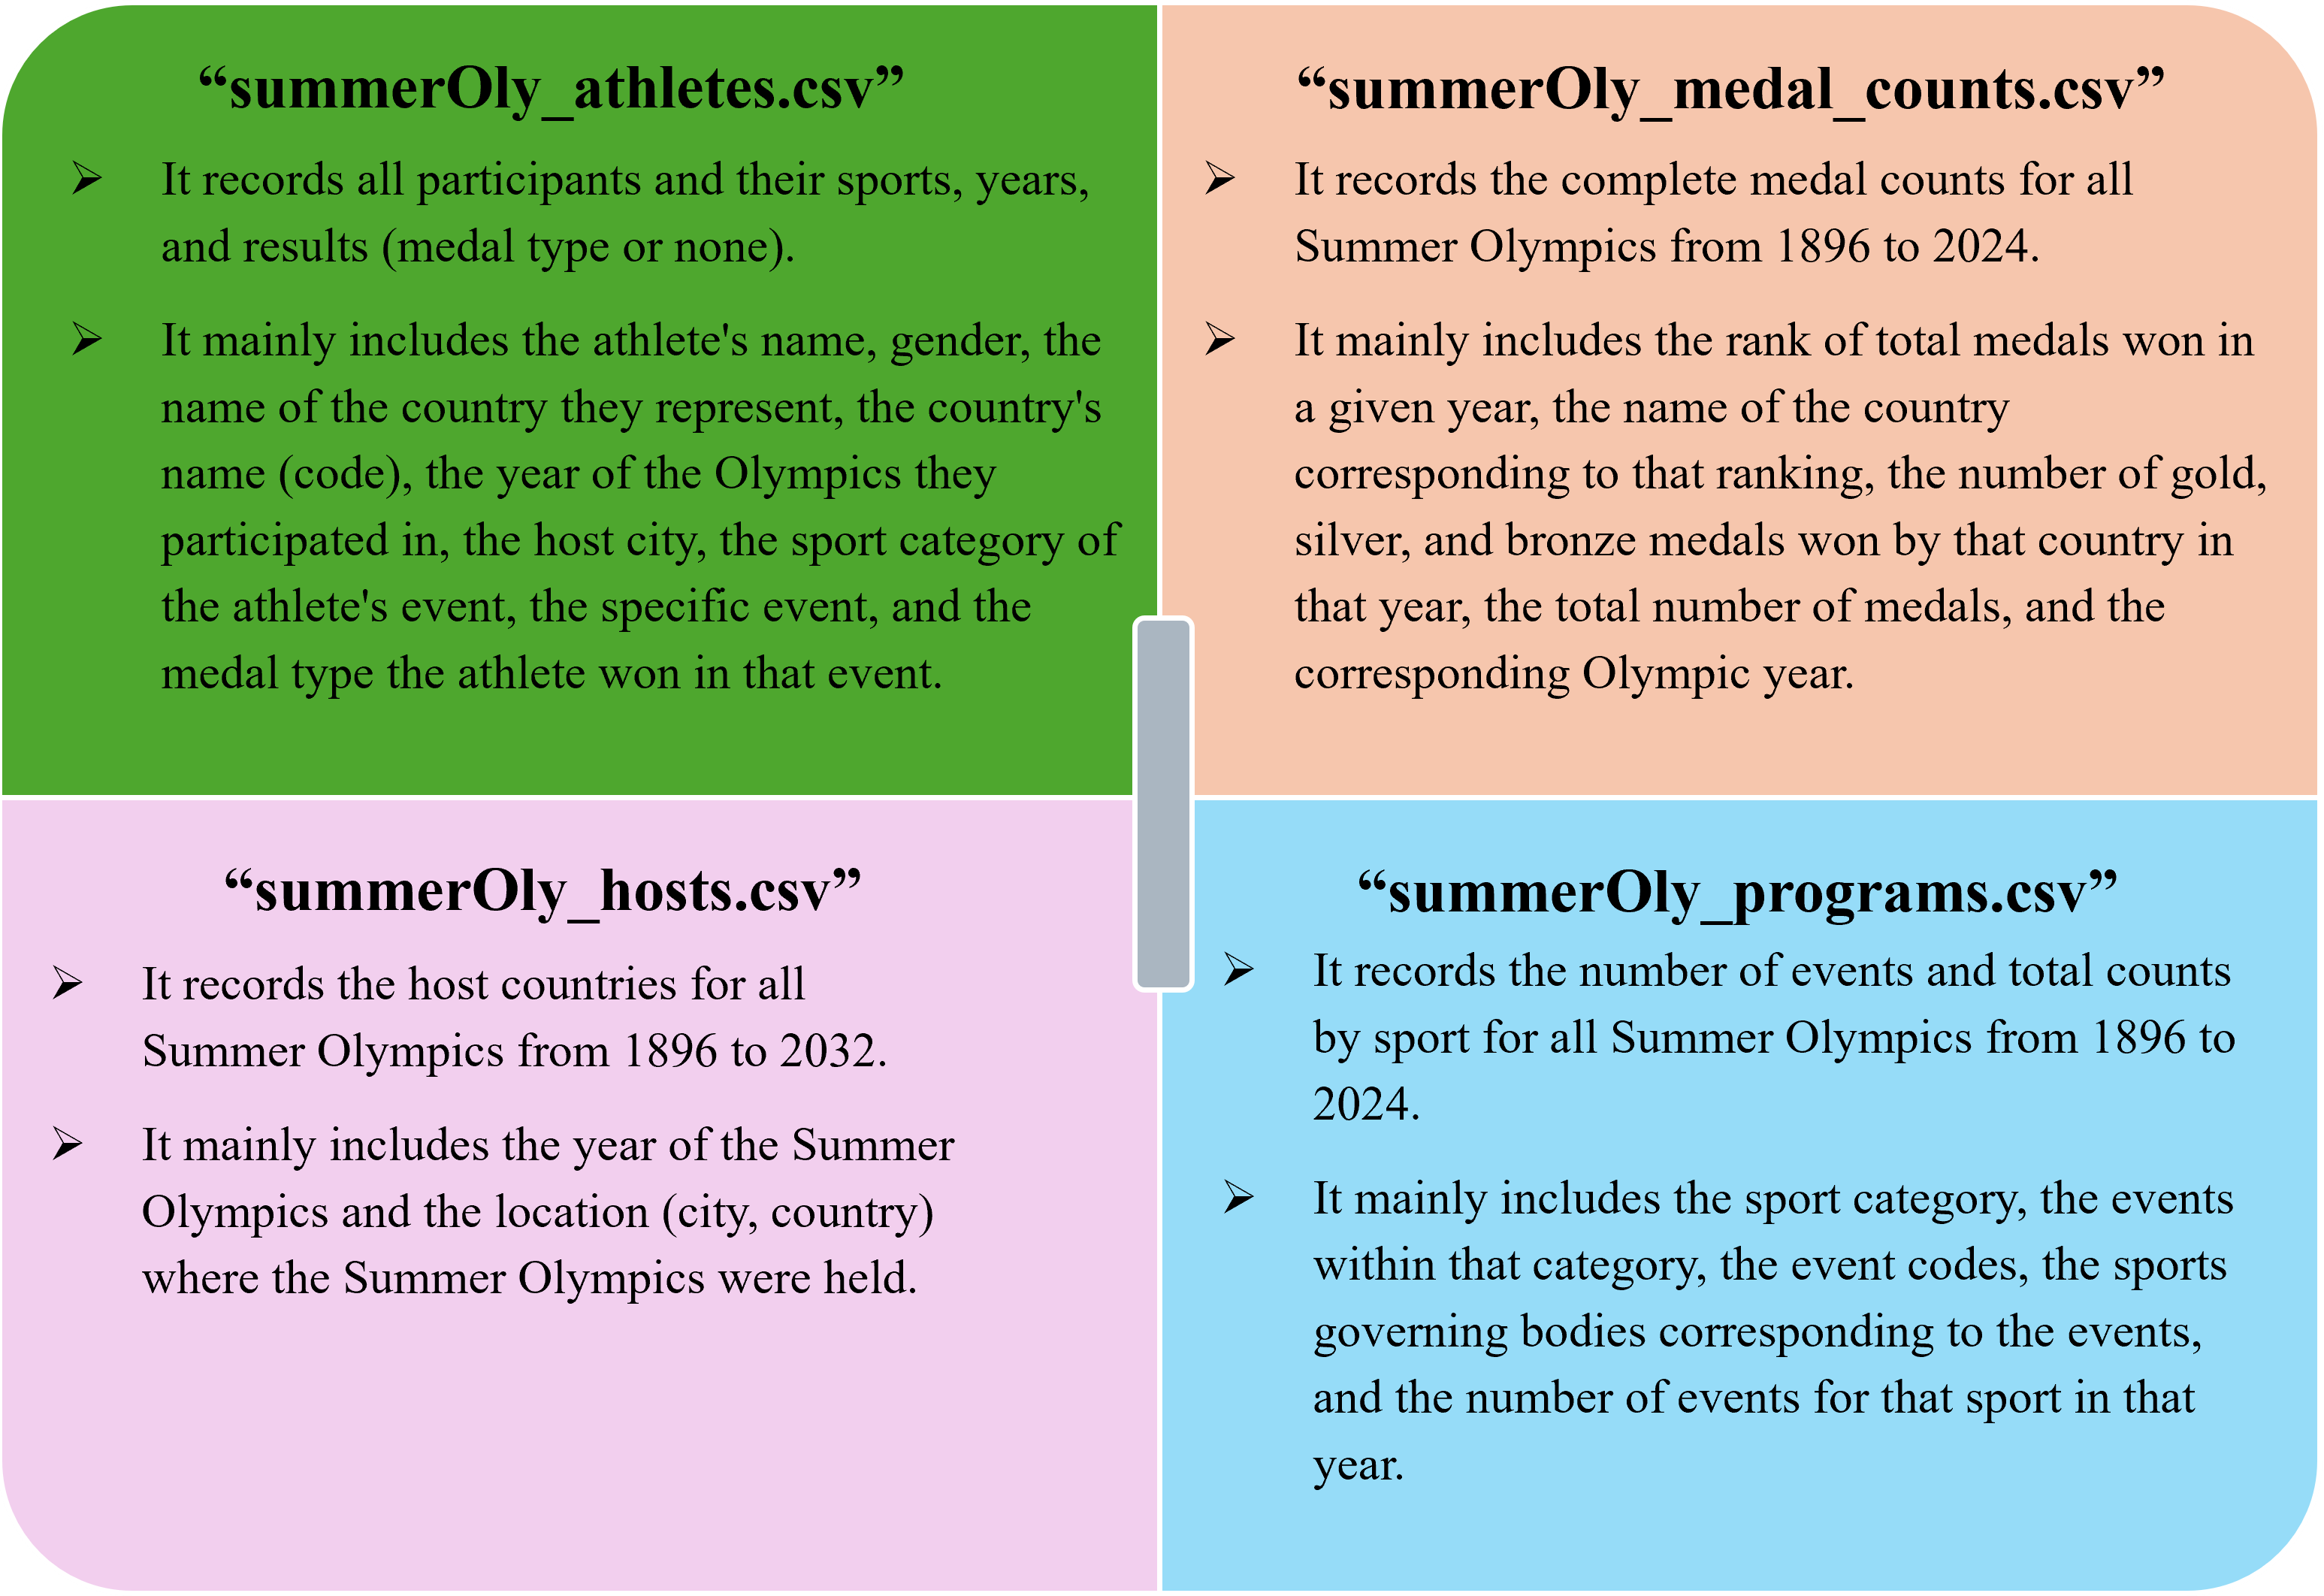
\includegraphics[width=10cm]{Overview of four data tables.png}
\caption{Overview of four data tables} \label{fig1}
\end{figure}

Notably: 

a) In 1936, during Nazi Germany, the Berlin Olympics was boycotted.

b) In 1980, during the Cold War, the Moscow Olympics was boycotted by the West. 

c) In 1984, during the Cold War, the Soviet Union boycotted the Los Angeles Olympics in the United States. 

These significant historical events caused large fluctuations in medal counts, resulting in some countries having zero medals, which can be analyzed further.

Encoding detection of the provided dataset files is shown in Table 1.

\begin{table}[h]
\centering
\caption{Data files and encoding formats}
\begin{tabular}{|l|l|} 
\hline
File                                  & Encoding                 \\ 
\hline
\textbf{data\_dictionary.csv}         & \textbf{windows 1252}    \\ 
\hline
\textbf{summerOly\_athletes.csv}      & \textbf{UTF-8}           \\ 
\hline
\textbf{summerOly\_hosts.csv}         & \textbf{UTF-8 with BOM}  \\ 
\hline
\textbf{summerOly\_medal\_counts.csv} & \textbf{UTF-8}           \\ 
\hline
\textbf{summerOly\_programs.csv}      & \textbf{windows 1252}    \\
\hline
\end{tabular}
\end{table}

For convenience in subsequent processing, the above files were uniformly converted to .xlsx files in UTF-8 encoding format.

\subsection{Data Cleaning}
Data cleaning was performed on the four data files: "summerOly_athletes.csv", "summerOly_hosts.csv", "summerOly_medal_counts.csv", and "summerOly_programs.csv". 
The specific steps are as follows:
\subsubsection{In "summerOly_athletes.csv" file}
\hskip\parindent a) There is an athlete named "671" in row 244172, which is clearly not a valid name. To facilitate subsequent unified processing, after checking other information about the athlete, the name was corrected to Liu Qinglian.

b)Duplicate value check revealed 1466 duplicate rows in the file, which have been deduplicated.

\begin{figure}[h] 
\centering
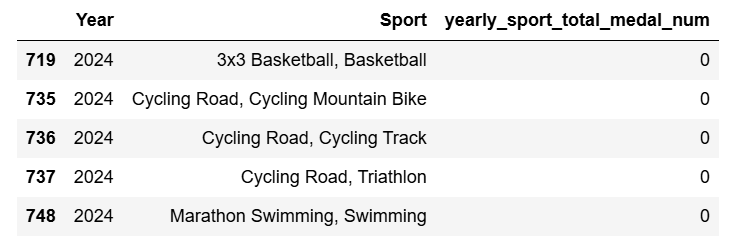
\includegraphics[width=0.8\linewidth]{The statistical situation of the abnormal Sport category.png}
\caption{The statistical situation of the abnormal Sport category} \label{fig1}
\end{figure}

\subsubsection{In "summerOly_programs.csv" file}
\hskip\parindent a) There are encoding issues, suspected to be due to encoding problems, so it was processed using the Windows 1252 encoding. 

b) There are missing values in the programs.csv file. The detailed missing situation is shown in Figure 2.

\begin{figure}[h] 
\centering
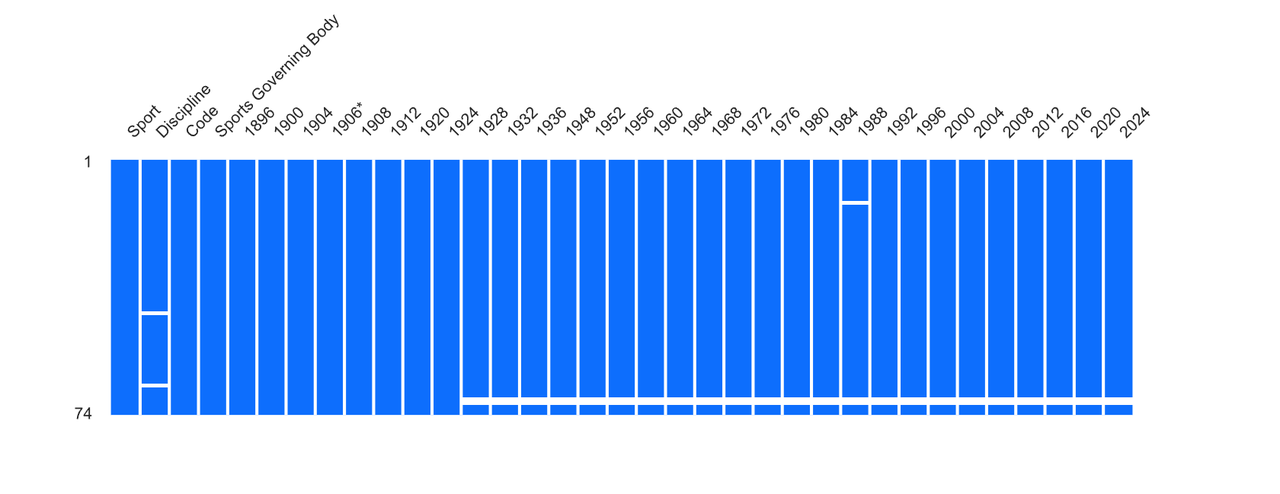
\includegraphics[width=10cm]{Schematic diagram of missing values in the programs table.PNG}
\caption{Schematic diagram of missing values in the programs table} \label{fig1}
\end{figure}
i.The value for 1988 in row 14 is missing.

ii.Figure skating and ice hockey, which are ice sports, were held at the Summer Olympics before 1924. However, they were moved to the first Winter Olympics in 1924, so the values for figure skating and ice hockey in rows 71 and 72 for 1924 and later are missing. 

iii.Because Modern Pentathlon and Water Motorsports do not have further classifications, the “Discipline” values are missing in rows 46 and 67. Based on other data analysis, the “Sport” values of the row was filled into the “Discipline” values. 

\subsubsection{In "summerOly_athletes.csv" and "summerOly_hosts.csv" files}
\hskip\parindent a)Datas for the year {1906} exist in “summerOly_athletes.csv” file but not in the hosts.csv file.

$\bigtriangleup$ Reason: According to research, an unofficial Olympics was held in Athens, Greece, in 1906. 

b)Datas for the years {2028, 2032, 1944, 1940, 1916} exist in “summerOly_hosts.csv” file but not in “summerOly_athletes.csv” file. 

$\bigtriangleup$ Reason: The Olympics for the years {2028, 2032} have not yet taken place. The host countries and cities have been determined, but the participating athletes have not been determined. The three Olympics originally scheduled for the years {1944, 1940, 1916} were canceled due to the two world wars in the 20th century. Although the hosts had been determined, there was no list of participating athletes because they could not be held.

\subsubsection{In "summerOly_medal_counts.csv" file}
\hskip\parindent After reading with UTF-8 encoding, it was found that the 'NOC' column had trailing spaces. All strings in this column were processed to remove excess leading and trailing spaces.

\section{Task 1:Development of the Medal Quantity Prediction Model}

\subsection{Sub-model I:A Multivariate Linear Regression-Based Model for Predicting the Total Medal Count of Countries in the Olympics}

\subsubsection{Model Preparation}
From the systematic analysis of influencing factors in the earlier stages, we know that the competitive performance of various countries in the Olympics, specifically quantified as the proportion of the total number of medals won in Olympic competitions, is closely related to the proportion of the total number of events in which the country participates in that year's Olympics. At the same time, the past performance of the country in the Olympics, especially in the previous year and recent years, has a significant and undeniable impact on the total number of medals for the current session.

Based on these factors, let $MP^{i}(t)$ represent the proportion of total medals won by the $i$-th country in the $t$-th Olympics; 


$i$

$t$

$S\!-\!Num^{i}(t)$

$P\!-\!Num^{i}(t)$

$Home^{i}(t)$

$Home^{i}(t)=1$

$S\_Num^{i}(t)$

$P\_Num^{i}(t)$

$S\_Num^{i}(t) = log(S\!-\!Num^{i}(t) + 1)$

$P\_Num^{i}(t) = log(P\!-\!Num^{i}(t) + 1)$

\begin{align} \label{eq1}
\notag
MP^{i}(t, \theta) = a_{1}^{i} + a_{2}^{i} \times S\_Num^{i}(t) + a_{3}^{i} \times P\_Num^i(t) \\ 
+ a_{4}^{i} \times Home^{i}(t) + a_{5}^{i} \times MP^{i}(t - 4) + \varepsilon^{i}(t)
\end{align}

$\theta = [a_{1}, a_{2}, a_{3}, a_{4}, a_{5}]$

$\varepsilon ^{i}(t)$

$t$

$y^{i}(t)$

$\hat{MP}^{i}(t, \hat{\theta })=\sum_{j=1}^{5}a_{j}^{i}\times f^{i}(t, j)$

\begin{figure}[h] 
\centering
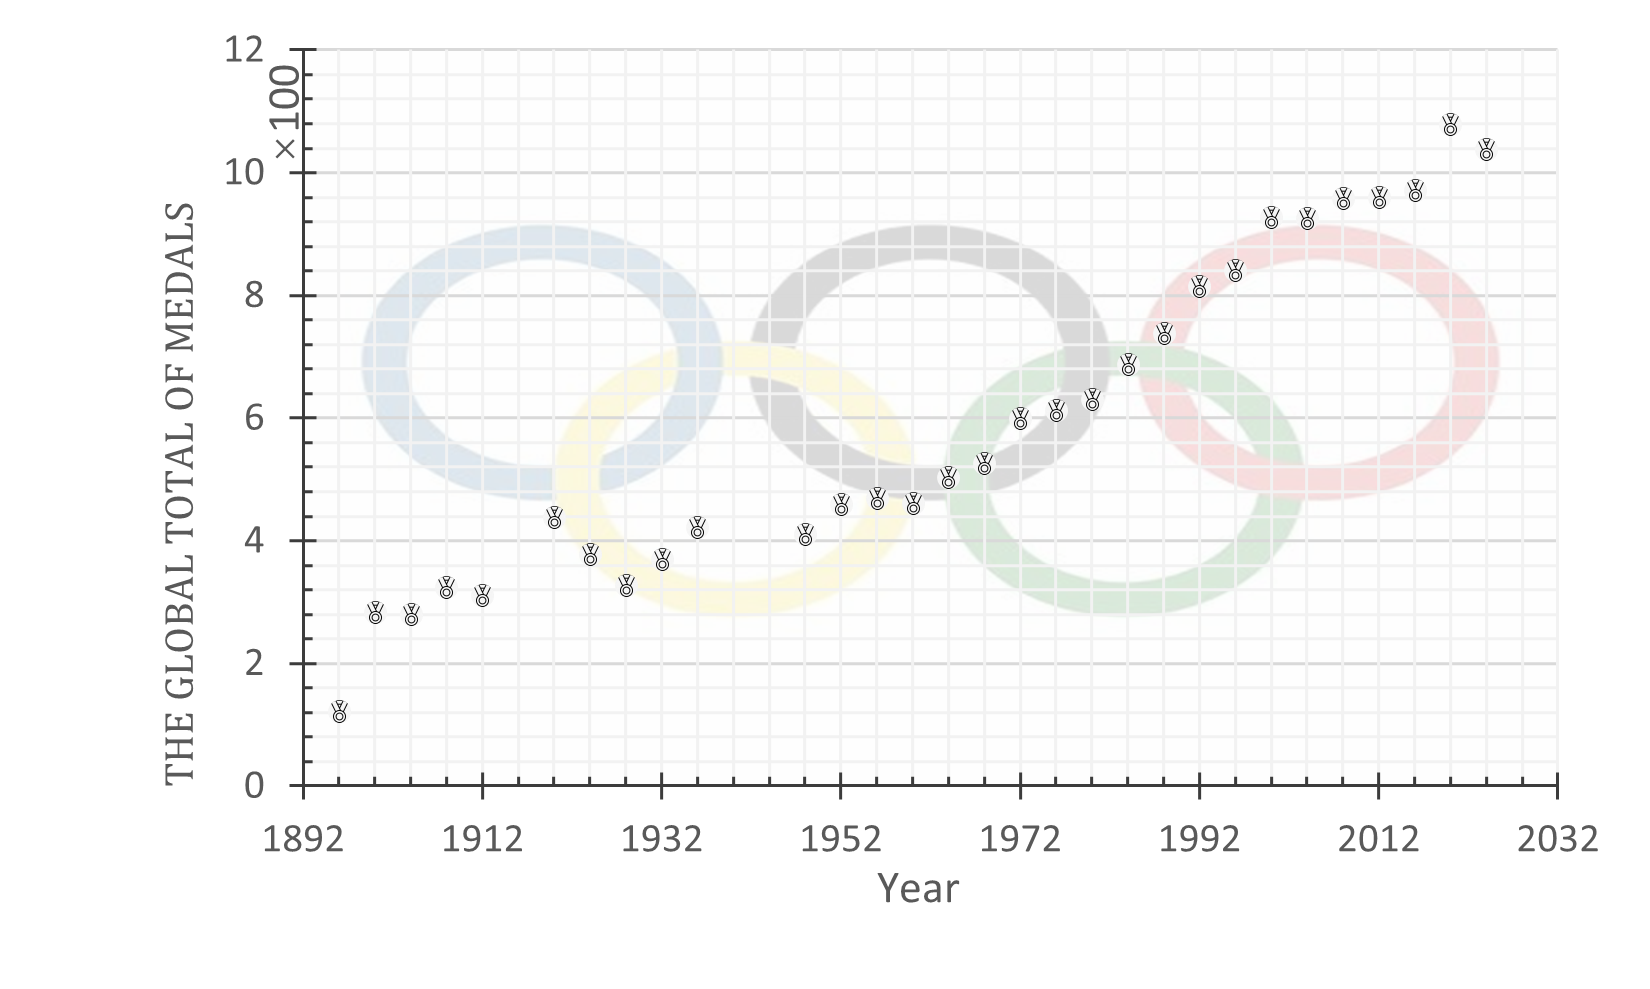
\includegraphics[width=10cm]{Global Total Olympic Medals Over Time.png}
\caption{Global Total Olympic Medals Over Time}
\end{figure}

$L(\hat{\theta }) = \sum_{t}[y^{i}(t)-\hat{M}^{i}(t, \hat{\theta})]^2$

$L(\hat{\theta })$

$\hat{\theta }$

\begin{equation}
M\_Sum = \beta_{0} + \beta_{1}t
\end{equation}

$\hat{\beta} = [\beta_{0}, \beta_{1}]$

$-1892$

$\hat{\beta}$

$\hat{\beta} = [131.282, 6.575]$

\begin{table}[h]
\centering
\caption{Data files and encoding formats}
\begin{tabular}{|c|c|c|} 
\hline
Year     & ~ 2028~~ & ~ 2032~~  \\ 
\hline
Pre\_Sum & 1026     & 1052      \\
\hline
\end{tabular}
\end{table}

\begin{equation}
\left\{\begin{array}{l}
m = min\left\{ k\in N: 1 - \frac{P(k + 1, \lambda ^{0}(t))}{P(k + 1)} \leq \frac{\alpha }{2}\right\}\\n = min\left\{ k\in N: \frac{P(k, \lambda ^{0}(t))}{P(k)} \leq \frac{\alpha }{2}\right\}
\end{array}\right.
\end{equation}

\begin{equation}
R^{2} = 1 - \frac{\sum_{i = 1}^{n}(F(t_{i}, \theta ) - F(t_{i}, \hat{\theta }))^2}{\sum_{i = 1}^{n}(F(t_{i}, \theta ) - \bar{F}(t_{i}, \hat{\theta }))^2}
\end{equation}


\begin{table}
\centering
\caption{prediction intervals for confidence}
\begin{tabular}{ccc} 
\toprule
alpha & min\_m & min\_n  \\ 
\toprule
0.05  & 29285  & 1       \\
0.10  & 29232  & 1       \\
0.25  & 29147  & 1       \\
\toprule
\end{tabular}
\end{table}

\subsection{Sub-model II : Adding Water Continuously}
\subsubsection{Model Preparation}
$N$ $X$ $Y$ $Z$

$N=X+Y+Z$

$S=W_{1}\times X+W_{2}\times Y+W_{3}\times Z$

$S=N$

$(X, Y, Z|N)\sim Multinomial(N, p_{1}, p_{2}, p_{3})$

$p_{1}$

$p_{2}$

$p_{3}$

$p_{1}+p_{2}+p_{3}=1$

$D^i(t)={X_{i}(t), Y_{i}(t), Z_{i}(t)}$

$i\in \{France, United States, Germany, Australia, ...\}$

$t\in \{1896, 1900, ...,2024\}$

$P(D_{i}|X_{i}, Y_{i}, Z_{i})= \prod_{t}(p(x_{i}(t), y_{i}(t), z_{i}(t)|X, Y, Z)$

$(x_{i}(t), y_{i}(t), z_{i}(t))$

$P(x^{i}(t), y^{i}(t), z^{i}(t)|N)=\frac{N!}{x^{i}!y^{i}!z^{i}!}P_{1} ^{x^{i}}P_{2} ^ {y^{i}}P_{3} ^ {z^{i}}$

$P(D|X, Y, Z)=\prod_{i=1}^{n}\frac{N!}{x^{i}!y^{i}!z^{i}!}P_{1}^{x^{i}}P_{2}^{y^{i}}P_{3}^{z^{i}}$

$\sum_{x+y+z=N}P(X=x, Y=y, Z=z|D)=1$

$P(X^{i}(t), Y^{i}(t), Z^{i}(t)|D) = \frac{1}{c} \times \frac{N!}{x!y!z!}P_{1}^{x}P_{2}^{y}P_{3}^{z}\prod_{t=1}^{n}\frac{N!}{x^{i}(t)!y^{i}(t)!z^{i}(t)!}P_{1}^{x^{i}(t)}P_{2}^{y^{i}(t)}P_{3}^{z^{i}(t)}$

Since we try to keep the temperature of the hot water in bathtub to be even, we have to derive the amount of inflow water and the energy dissipated by the hot water into the air.

We derive the basic convection heat transfer control equations based on the former scientists’ achievement. Then, we define the mean temperature of bath water. Afterwards, we determine two types of heat transfer: the boundary heat transfer and the evaporation heat transfer. Combining thermodynamic formulas, we derive calculating results. Via Fluent software, we get simulation results.

\subsection{Control Equations and Boundary Conditions}

According to thermodynamics knowledge, we recall on basic convection
heat transfer control equations in rectangular coordinate system. Those
equations show the relationship of the temperature of the bathtub water in space.

We assume the hot water in the bathtub as a cube. Then we put it into a
rectangular coordinate system. The length, width, and height of it is $a,\, b$ and $c$.

\begin{figure}[h] 
\centering
\includegraphics[width=8cm]{fig2.jpg}
\caption{Modeling process} \label{fig2}
\end{figure}

In the basis of this, we introduce the following equations \cite{5}:

\begin{itemize}
\item {\bf Continuity equation:}
\end{itemize}

\begin{equation} \label{eq1}
\frac{\partial u}{\partial x} + \frac{\partial v}{\partial y} +\frac{\partial w}{\partial z} =0
\end{equation}

\noindent where the first component is the change of fluid mass along the $X$-ray. The second component is the change of fluid mass along the $Y$-ray. And the third component is the change of fluid mass along the $Z$-ray. The sum of the change in mass along those three directions is zero.

\begin{itemize}
\item {\bf Moment differential equation (N-S equations):}
\end{itemize}

\begin{equation} \label{eq2}
\left\{
\begin{array}{l} \!\!
\rho \Big(u \dfrac{\partial u}{\partial x} + v \dfrac{\partial u}{\partial y} + w\dfrac{\partial u}{\partial z} \Big) = -\dfrac{\partial p}{\partial x} + \eta \Big(\dfrac{\partial^2 u}{\partial x^2} + \dfrac{\partial^2 u}{\partial y^2} + \dfrac{\partial^2 u}{\partial z^2} \Big) \\[0.3cm]
\rho \Big(u \dfrac{\partial v}{\partial x} + v \dfrac{\partial v}{\partial y} + w\dfrac{\partial v}{\partial z} \Big) = -\dfrac{\partial p}{\partial y} + \eta \Big(\dfrac{\partial^2 v}{\partial x^2} + \dfrac{\partial^2 v}{\partial y^2} + \dfrac{\partial^2 v}{\partial z^2} \Big) \\[0.3cm]
\rho \Big(u \dfrac{\partial w}{\partial x} + v \dfrac{\partial w}{\partial y} + w\dfrac{\partial w}{\partial z} \Big) = -g-\dfrac{\partial p}{\partial z} + \eta \Big(\dfrac{\partial^2 w}{\partial x^2} + \dfrac{\partial^2 w}{\partial y^2} + \dfrac{\partial^2 w}{\partial z^2} \Big)  
\end{array}
\right.
\end{equation}

\begin{itemize}
\item {\bf Energy differential equation:}
\end{itemize}

\begin{equation} \label{eq3}
\rho c_p \Big( u\frac{\partial t}{\partial x} + v\frac{\partial t}{\partial y} + w\frac{\partial t}{\partial z} \Big) = \lambda \Big(\frac{\partial^2 t}{\partial x^2} + \frac{\partial^2 t}{\partial y^2} + \frac{\partial^2 t}{\partial z^2} \Big)
\end{equation}

\noindent where the left three components are convection terms while the right three components are conduction terms.

By Equation \eqref{eq3}, we have ......

......

On the right surface in Fig. \ref{fig2}, the water also transfers heat firstly with bathtub inner surfaces and then the heat comes into air. The boundary condition here is ......

\subsubsection{Definition of the Mean Temperature}

......

\subsubsection{Determination of Heat Transfer Capacity}

......

\subsection{Sub-model III: Adding Water Discontinuously}
$P\_Num^{i}(t)$

$P_{1}\_Num^{i}(t) = P+P\_Num^{i}(t)$

$P$

$S\_Num^{i}(t)$

\begin{equation}
S_{1}\_Num^{i}(t) = S\_Num^{i}(t) + f(p)
\end{equation}

$f(p) = \sum_{k=1}^{n}w_{k}I_{k}$

$w_{k}$

$I_{k}$

$MP^{i}(t, \theta) = a_{1}^{i}+a_{2}^{i}\times S_{1}\_Num^{i}(t) + a_{3}^{i}\times P_{1}\_Num^{i}(t) + a_{4}^{i}\times H^{i}(t) + a_{5}^{i}MP^{i}(t-4)$

$X^{i}(t)$

$Y^{i}(t)$

$Z^{i}(t)$

$P_{1}^{i}(t)$

$P_{2}^{i}(t)$

$P_{3}^{i}(t)$

$f(M)$

$P_{j}^{oi}(t) = P_{j}^{i}(t)f(M)$

$p_{1}$

$Me^{i}\times p_{1}^{i}$

In order to establish the unsteady sub-model, we recall on the working principle of air conditioners. The heating performance of air conditions consist of two processes: heating and standby. After the user set a temperature, the air conditioner will begin to heat until the expected temperature is reached. Then it will go standby. When the temperature get below the expected temperature, the air conditioner begin to work again. As it works in this circle, the temperature remains the expected one.

Inspired by this, we divide the bathtub working into two processes: adding
hot water until the expected temperature is reached, then keeping this
condition for a while unless the temperature is lower than a specific value. Iterating this circle ceaselessly will ensure the temperature kept relatively stable.

\subsection{Heating Model}

\subsubsection{Control Equations and Boundary Conditions}

\subsubsection{Determination of Inflow Time and Amount}

\subsection{Standby Model}

\subsection{Results}

\quad~ We first give the value of parameters based on others’ studies. Then we get the calculation results and simulating results via those data.

\subsubsection{Determination of Parameters}

After establishing the model, we have to determine the value of some
important parameters.

As scholar Beum Kim points out, the optimal temperature for bath is
between 41 and 45$^\circ$C [1]. Meanwhile, according to Shimodozono's study, 41$^\circ$C warm water bath is the perfect choice for individual health [2]. So it is reasonable for us to focus on $41^\circ$C $\sim 45^\circ$C. Because adding hot water continuously is a steady process, so the mean temperature of bath water is supposed to be constant. We value the temperature of inflow and outflow water with the maximum and minimum temperature respectively.

The values of all parameters needed are shown as follows:

.....

\subsubsection{Calculating Results}

Putting the above value of parameters into the equations we derived before, we can get the some data as follows:

%%普通表格
\begin{table}[h]  %h表示固定在当前位置
\centering        %设置居中
\caption{The calculating results}  %表标题
\vspace{0.15cm}
\label{tab2}                       %设置表的引用标签
\begin{tabular}{|c|c|c|}  %3个c表示3列, |可选, 表示绘制各列间的竖线
\hline                    %画横线
Variables & Values & Unit     \\ \hline  %各列间用&隔开
$A_1$     & 1.05   &   $m^2$  \\ \hline
$A_2$     & 2.24   &   $m^2$  \\ \hline
$\Phi_1$  & 189.00 &   $W$   \\ \hline
$\Phi_2$  & 43.47  &   $W$   \\ \hline
$\Phi$    & 232.47 &   $W$   \\ \hline
$q_m$     & 0.014  &   $g/s$ \\ \hline
\end{tabular}
\end{table}

From Table \ref{tab2}, ......

......

\section{Correction and Contrast of Sub-Models}

$P_{i, j}(t) = M_{i, j}(t) / S_{i, j}(t)$

$P_{i, j}(t)$

$M_{i, j}(t)$

$S_{i, j}(t)$

$\Delta P_{i, j} = P_{i, j}(t_{1}) - p_{i, j}(t_{0})$

$\Delta P_{i, j} = \bar{p}_{i, j}^{after}(t_{0}) - \bar{p}_{i, j}^{before}(t_{0})$

$\Delta M_{i, j}(t) = \Delta P_{i, j} \times A_{i, j}(t)$

$\Delta P_{i, j}$

$MP^{i} = a_{1} ^ {i} + a_{2} ^{i}\times S_{1}\_Num^{i} + a_{3}^{i}\times P_{1}\_Num^{i} + a_{5}^{i}M$

$P_{1}\_Num^{i}=P_{ij} + \Delta P_{i, j} + P\_Num^{i}$

$\Delta M=M_{c} - M_{b}$
After establishing two basic sub-models, we have to correct them in consideration of evaporation heat transfer. Then we define two evaluation criteria to compare the two sub-models in order to determine the optimal bath strategy.

\subsection{Correction with Evaporation Heat Transfer}

Someone may confuse about the above results: why the mass flow in the first sub-model is so small? Why the standby time is so long? Actually, the above two sub-models are based on ideal conditions without consideration of the change of boundary conditions, the motions made by the person in bathtub and the evaporation of bath water, etc. The influence of personal motions will be discussed later. Here we introducing the evaporation of bath water to correct sub-models.

\subsection{Contrast of Two Sub-Models}

Firstly we define two evaluation criteria. Then we contrast the two submodels via these two criteria. Thus we can derive the best strategy for the person in the bathtub to adopt.

\section{Model Sensitivity Analysis}

\subsection{The Influence of Different Bathtubs}

Definitely, the difference in shape and volume of the tub affects the
convection heat transfer. Examining the relationship between them can help
people choose optimal bathtubs.

\subsubsection{Different Volumes of Bathtubs}

In reality, a cup of water will be cooled down rapidly. However, it takes quite long time for a bucket of water to become cool. That is because their volume is different and the specific heat of water is very large. So that the decrease of temperature is not obvious if the volume of water is huge. That also explains why it takes 45 min for 320 L water to be cooled by 1$^\circ$C.

In order to examine the influence of volume, we analyze our sub-models
by conducting sensitivity Analysis to them.

We assume the initial volume to be 280 L and change it by $\pm 5$\%, $\pm 8$\%, $\pm 12$\% and $\pm 15$\%. With the aid of sub-models we established before, the variation of some parameters turns out to be as follows

%%三线表
\begin{table}[h] %h表示固定在当前位置
\centering  %设置居中
\caption{Variation of some parameters}  %表标题
\label{tab7} %设置表的引用标签
\begin{tabular}{ccccccc} %7个c表示7列, c表示每列居中对齐, 还有l和r可选
\toprule  %画顶端横线
$V$      & $A_1$   & $A_2$   & $T_2$    & $q_{m1}$ & $q_{m2}$ & $\Phi_q$ \\
\midrule  %画中间横线
-15.00\% & -5.06\% & -9.31\% & -12.67\% & -2.67\%  & -14.14\% & -5.80\% \\
-12.00\% & -4.04\% & -7.43\% & -10.09\% & -2.13\%  & -11.31\% & -4.63\% \\
-8.00\%  & -2.68\% & -4.94\% & -6.68\%  & -1.41\%  & -7.54\%  & -3.07\% \\
-8.00\%  & -2.68\% & -4.94\% & -6.68\%  & -1.41\%  & -7.54\%  & -3.07\% \\
-8.00\%  & -2.68\% & -4.94\% & -6.68\%  & -1.41\%  & -7.54\%  & -3.07\% \\
-8.00\%  & -2.68\% & -4.94\% & -6.68\%  & -1.41\%  & -7.54\%  & -3.07\% \\
-8.00\%  & -2.68\% & -4.94\% & -6.68\%  & -1.41\%  & -7.54\%  & -3.07\% \\
-8.00\%  & -2.68\% & -4.94\% & -6.68\%  & -1.41\%  & -7.54\%  & -3.07\% \\
-8.00\%  & -2.68\% & -4.94\% & -6.68\%  & -1.41\%  & -7.54\%  & -3.07\% \\
-8.00\%  & -2.68\% & -4.94\% & -6.68\%  & -1.41\%  & -7.54\%  & -3.07\% \\
-8.00\%  & -2.68\% & -4.94\% & -6.68\%  & -1.41\%  & -7.54\%  & -3.07\% \\
\bottomrule  %画底部横线
\end{tabular}
\end{table}

\section{Model Assessment}

\subsection{Strengths}

\begin{itemize}
\item We analyze the problem based on thermodynamic formulas and laws, so that the model we established is of great validity.

\item Our model is fairly robust due to our careful corrections in consideration of real-life situations and detailed sensitivity analysis.

\item Via Fluent software, we simulate the time field of different areas throughout the bathtub. The outcome is vivid for us to understand the changing process.

\item We come up with various criteria to compare different situations, like water consumption and the time of adding hot water. Hence an overall comparison can be made according to these criteria.

\item Besides common factors, we still consider other factors, such as evaporation and radiation heat transfer. The evaporation turns out to be the main reason of heat loss, which corresponds with other scientist’s experimental outcome.
\end{itemize}

\subsection{Weaknesses}

\begin{itemize}
\item Having knowing the range of some parameters from others’ essays, we choose a value from them to apply in our model. Those values may not be reasonable in reality.

\item Although we investigate a lot in the influence of personal motions, they are so complicated that need to be studied further.

\item Limited to time, we do not conduct sensitivity analysis for the influence of personal surface area.
\end{itemize}

\section{Further Discussion}

In this part, we will focus on different distribution of inflow faucets. Then we discuss about the real-life application of our model.

\begin{itemize}
\item Different Distribution of Inflow Faucets

In our before discussion, we assume there being just one entrance of inflow.

From the simulating outcome, we find the temperature of bath water is hardly even. So we come up with the idea of adding more entrances.

The simulation turns out to be as follows

\begin{figure}[h] 
\centering
\includegraphics[width=12cm]{fig24.jpg}
\caption{The simulation results of different ways of arranging entrances} \label{fig24}
\end{figure}

From the above figure, the more the entrances are, the evener the temperature will be. Recalling on the before simulation outcome, when there is only one entrance for inflow, the temperature of corners is quietly lower than the middle area.

In conclusion, if we design more entrances, it will be easier to realize the goal to keep temperature even throughout the bathtub.

\item Model Application

Our before discussion is based on ideal assumptions. In reality, we have to make some corrections and improvement.

\begin{itemize}
\item[1)] Adding hot water continually with the mass flow of 0.16 kg/s. This way can ensure even mean temperature throughout the bathtub and waste less water.

\item[2)] The manufacturers can design an intelligent control system to monitor the temperature so that users can get more enjoyable bath experience.

\item[3)] We recommend users to add bubble additives to slow down the water being cooler and help cleanse. The additives with lower thermal conductivity are optimal.

\item[4)] The study method of our establishing model can be applied in other area relative to convection heat transfer, such as air conditioners.
\end{itemize}
\end{itemize}

\begin{thebibliography}{99}
\addcontentsline{toc}{section}{Reference}

\bibitem{1} Gi-Beum Kim. Change of the Warm Water Temperature for the Development of Smart Healthecare Bathing System. Hwahak konghak. 2006, 44(3): 270-276.
\bibitem{2} \url{https://en.wikipedia.org/wiki/Convective_heat_transfer#Newton.27s_law_of_cooling}
\bibitem{3} \url{https://en.wikipedia.org/wiki/Navier\%E2\%80\%93Stokes_equations}
\bibitem{4} \url{https://en.wikipedia.org/wiki/Computational_fluid_dynamics}
\bibitem{5} Holman J P. Heat Transfer (9th ed.), New York: McGraw-Hill, 2002. 
\bibitem{6} Liu Weiguo, Chen Zhaoping, ZhangYin. Matlab program design and application. Beijing: Higher education press, 2002. (In Chinese)

\end{thebibliography}

\newpage

\begin{letter}{Enjoy Your Bath Time!}

From simulation results of real-life situations, we find it takes a period of time for the inflow hot water to spread throughout the bathtub. During this process, the bath water continues transferring heat into air, bathtub and the person in bathtub. The difference between heat transfer capacity makes the temperature of various areas to be different. So that it is difficult to get an evenly maintained temperature throughout the bath water.

In order to enjoy a comfortable bath with even temperature of bath water and without wasting too much water, we propose the following suggestions.

\begin{itemize}
\item Adding hot water consistently
\item Using smaller bathtub if possible
\item Decreasing motions during bath
\item Using bubble bath additives
\item Arranging more faucets of inflow
\end{itemize}

\vspace{\parskip}

Sincerely yours,

Your friends

\end{letter}

\newpage

\begin{appendices}

\section{First appendix}

In addition, your report must include a letter to the Chief Financial Officer (CFO) of the Goodgrant Foundation, Mr. Alpha Chiang, that describes the optimal investment strategy, your modeling approach and major results, and a brief discussion of your proposed concept of a return-on-investment (ROI). This letter should be no more than two pages in length.

Here are simulation programmes we used in our model as follow.\\

\textbf{\textcolor[rgb]{0.98,0.00,0.00}{Input matlab source:}}
\lstinputlisting[language=Matlab]{./code/mcmthesis-matlab1.m}

\section{Second appendix}

some more text \textcolor[rgb]{0.98,0.00,0.00}{\textbf{Input C++ source:}}
\lstinputlisting[language=C++]{./code/mcmthesis-sudoku.cpp}

\end{appendices}
\end{document}
%%
%% This work consists of these files mcmthesis.dtx,
%%                                   figures/ and
%%                                   code/,
%% and the derived files             mcmthesis.cls,
%%                                   mcmthesis-demo.tex,
%%                                   README,
%%                                   LICENSE,
%%                                   mcmthesis.pdf and
%%                                   mcmthesis-demo.pdf.
%%
%% End of file `mcmthesis-demo.tex'.
